\documentclass[12pt,spanish,fleqn,letterpaper]{scrbook}

\usepackage[utf8]{inputenc}
\usepackage[spanish]{babel}
%\usepackage{scrlayer-scrpage}
\usepackage{epsfig}
\usepackage{epic}
\usepackage{eepic}
\usepackage{fancyhdr}
\usepackage{amsmath}
\usepackage{amsfonts}
\usepackage{threeparttable}
\usepackage{amscd}
\usepackage{here}
\usepackage{graphicx}
\usepackage{lscape}
\usepackage{tabularx}
\usepackage{subcaption}
\usepackage{longtable}
\usepackage{cite}
\usepackage{scrhack}
\usepackage{tikz}

\usepackage{comment} %comentarios


% Manejo de hypervínculos
\usepackage{hyperref}
\hypersetup{bookmarksnumbered=true,
            colorlinks=true,
            citecolor=black,
            linkcolor=black}
            
% *** GRAPHICS RELATED PACKAGES ***
\usepackage{epstopdf}
 \usepackage[siunitx, american, smartlabels, cute inductors, europeanvoltages]{circuitikz}
\usetikzlibrary{shapes.geometric}
\usetikzlibrary{arrows.meta,backgrounds}
\usetikzlibrary{decorations.pathreplacing}
\usetikzlibrary{chains}
\usetikzlibrary{calc}
\makeatletter
\ctikzset{lx/.code args={#1 and #2}{ 
  \pgfkeys{/tikz/circuitikz/bipole/label/name=\parbox{1cm}{\centering #1  \\ #2}}
    \ctikzsetvalof{bipole/label/unit}{}
    \ifpgf@circ@siunitx 
        \pgf@circ@handleSI{#2}
        \ifpgf@circ@siunitx@res 
            \edef\pgf@temp{\pgf@circ@handleSI@val}
            \pgfkeyslet{/tikz/circuitikz/bipole/label/name}{\pgf@temp}
            \edef\pgf@temp{\pgf@circ@handleSI@unit}
            \pgfkeyslet{/tikz/circuitikz/bipole/label/unit}{\pgf@temp}
        \else
        \fi
    \else
    \fi
}}

%Estilo de los encabezados
%Options: Sonny, Lenny, Glenn, Conny, Rejne, Bjarne, Bjornstrup
\usepackage[Bjornstrup]{fncychap}

%Para rotar texto, objetos y tablas
\usepackage{rotating} 

% Como numerar las ecuaciones, figuras y tablas
\renewcommand{\theequation}{\thechapter-\arabic{equation}}
\renewcommand{\thefigure}{\textbf{\thechapter-\arabic{figure}}}
\renewcommand{\thetable}{\textbf{\thechapter-\arabic{table}}}

%% Estilo de las páginas

\KOMAoptions{DIV=14}%Margenes 4-15 (menos numero es menos margen)
%\usepackage{showframe}

\KOMAoptions{headlines=2.1}
\KOMAoptions{footsepline=true}

\recalctypearea
 \fancyhead[RE]{\itshape\nouppercase puto}
 \fancyhead[LO]{\itshape\nouppercase\rightmark}
 \fancyfoot[C]{\thepage}
 

% Unidades de separación
\unitlength1mm %Define la unidad LE para Figuras
\mathindent0cm %Define la distancia de las formulas al texto
\marginparwidth0cm
\parindent0cm %Define la distancia de la primera linea de un parrafo

%Para tablas,  redefine el backschlash en tablas donde se define la posición del texto en las
%casillas (con \centering \raggedright o \raggedleft)
\newcommand{\PreserveBackslash}[1]{\let\temp=\\#1\let\\=\temp}
\let\PBS=\PreserveBackslash

%Espacio entre lineas
\renewcommand{\baselinestretch}{1.1}

% Array modificado
\newcommand{\arr}[1]{\raisebox{1.5ex}[0cm][0cm]{#1}}

%Definir comandos nuevos
\usepackage{Encabezado/Befehle}


%separación de silabas de palabras mal cortadas entre líneas
\hyphenation {pu-to}
%\includeonly{Kap1/Kap1,Kap2/Kap2}
\begin{document}
\pagenumbering{roman}
%\newpage
%\setcounter{page}{1}

\begin{titlepage}
\begin{center}
%\begin{tabular}{ccc}
%img izq &  & img der
%\end{tabular} 
\Large{\textbf{Universidad Nacional de San Agustín} }\\ 
\Large{\textbf{Facultad de Ingenieria de produccion y servicios}} \\
\large{\textbf{Escuela profesional de Ciencia de la computación}} \\
%\large{\textbf{Datos adicionales ..}} \\\vskip 1cm
\centerline{\resizebox{!}{50mm}{\rotatebox{0}{
\includegraphics{HojaTitulo/unsa.pdf}}}}
\huge{\textbf{``Metodo Spatio-temporal para la detección y registro de acciones humanas en video de poca resolucion."}} \\ \vskip 1cm
 \large{ Tesis que para obtener el título de}\\
 \large{\textbf{Licenciado en Ciencia de la computación}}\\  \vskip 1cm
 \large{Presenta:}\\ 
 \large{\textbf{Luigy Alex Machaca Arcana}}\\ \vskip 1cm
 \large{Asesores:}\\
 \large{\textbf{Juan Carlos Gutierrez Cáceres}}\\
 \large{\textbf{Alvaro Mamani Aliaga}} \\ \vskip .5cm
 \large{24 junio 2017} 
\end{center}
\end{titlepage}

%Se pueden incluir tantas páginas iniciales se requieran cada una dentro del entorno \begin{titlepage} \end{titlepage}
\newpage
\newpage
\thispagestyle{empty} \vspace*{10ex} \textbf{\centerline{\LARGE
Declaraci\'{o}n}}\normalsize\\\\\\%
Me permito afirmar que he realizado la presente tesis de manera aut\'{o}noma y con la \'{u}nica ayuda de los medios permitidos y no diferentes a los mencionados en la propia tesis. Todos los pasajes
que se han tomado de manera textual o figurativa de textos publicados y no publicados, los he reconocido en el presente trabajo. Ninguna parte del presente trabajo se ha empleado en ning\'{u}n otro tipo de tesis.
\\\\%
Arequipa, Perú, 23.07.2017
\\\\%
\\\\%
\\
\rule{6cm}{0.5pt}\\
(Luigy Alex Machaca Arcana)
\thispagestyle{empty} \vspace*{10ex} \textbf{\centerline{\LARGE
Abstract}}\normalsize\\\\\\%
El reconocimiento de movimiento y acciones para video-vigilancia es un campo activo de visión computacional. Hoy en dìa, existen varias técnicas que intentan abordar este tema, algunos mediante, mapeo 3D con un alto costo computacional. Este artículo describe algoritmos de software que pueden detectar a las personas en la escena y analizar diferentes acciones y patrones de movimiento en tiempo real.\\
 
La motivación para este trabajo es crear un sistema capaz de poder acciones violentas en videos de vigilancia, sin la necesidad de asistencia humana para la detección de dichos actos.\\
 
Utilizamos un método para la segmentación del primer plano y del fondo, crearemos un vector caracteristico para discriminar y seguir a varias personas de la escena. Finalmente, se describe un simple algoritmo basado en MVFI para discriminar acciones y movimientos corporales a través de la magnitud de la velocidad y la dirección en la cual se detecta el movimiento de píxeles.


\newpage
%%%%%%%%%%%%%%%%%%%%%%%%%%%%%%%%

\begin{comment}


ESTRUCTURA  TESIS \\
------------------\\
cap1 - introducción

\begin{itemize}
\item concepto y motivación
\item descripción del problema
\item objetivos
  \begin{itemize}
  \item generales
  \item especificos
  \end{itemize}
\item estructura del documento
\end{itemize}

cap2 - trabajos relacionados
\begin{itemize}
\item consideraciones iniciales
\item descripción de trabajos
\item comparación de trabajos
\item consideraciones finales
\end{itemize}

cap3 marco teorico
-------
\begin{itemize}
\item no sé q irá aqui...
\end{itemize}
\end{comment}


\renewcommand{\tablename}{\textbf{Tabla}}
\renewcommand{\figurename}{\textbf{Figura}}
\renewcommand{\listtablename}{Lista de Tablas}
\renewcommand{\listfigurename}{Lista de Figuras}
\renewcommand{\contentsname}{Contenido}


%\newcommand{\clearemptydoublepage}{\newpage{\pagestyle{empty}\cleardoublepage}}

\tableofcontents
%\newcommand{\clearemptydoublepage}{\newpage{\pagestyle{empty}\cleardoublepage}}
\chapter*{Lista de símbolos}
\addcontentsline{toc}{chapter}{\numberline{}Lista de símbolos}
\begin{comment}
Esta sección se incluyen símbolos generales (con letras latinas y griegas), subíndices, superíndices y abreviaturas (incluir sólo las clases de símbolos que se utilicen). Cada una de estas listas debe estar ubicada en orden alfabético de acuerdo con la primera letra del símbolo.
\end{comment}


\begin{comment}

\section*{Símbolos con letras latinas}
 \label{simbolos}
 \renewcommand{\arraystretch}{1.3}
\begin{longtable}[l]{>{$}l<{$}l>{$}l<{$}>{$}l<{$}}
%\begin{tabular}
\textbf{Símbolo}&\textbf{Término}&\textbf{Unidad SI}&\textbf{Definición}\\[0.5ex]\hline
\endfirsthead%
\textbf{Símbolo}&\textbf{Término}&\textbf{Unidad SI}&\textbf{Definición}\\[0.5ex]\hline
\endhead%
      A              &Área                                   &\text{m}^{2}                         &\int\int dxdy\\%
      A_{\text{BET}} &Área interna del sólido                &\frac{\text{m}^{2}}{\text{g}}        &\text{ver DIN ISO 9277}\\%
      A_{\text{g}}   &Área transversal de la fase gaseosa    &\text{m}^{2}                         &\text{Ec...}\\%
      A_{\text{s}}   &Área transversal de la carga a granel  &\text{m}^{2}                         &\text{Ec...}\\%
      a              &Coeficiente                            &1                                    &\text{Ec...}\\%
      a              &Contenido de ceniza                    &1                                    &\frac{m_{\text{ceniza}}}{m_{\text{bm,0}}}\\%
      c              &Contenido de carbono                   &1                                    &\frac{m_{\text{C}}}{m}\\%
      c              &Longitud de la cuerda                  &\text{m}                             &\text{Figura...}\\
      c              &Concentración de la cantidad de materia&\frac{\text{mol}}{\text{m}^{3}}      &\frac{n}{V}\\%
      D              &Diámetro                               &\text{m}                             &\\%
      E_{\text{A}}   &Energía de activación                  &\frac{\text{kJ}}{\text{mol}}         &\text{Ec....}\\%
      F              &Fracción de materia volátil            &1                                    &\text{ver DIN 51720}\\%
      Fr             &N\'{u}mero de Froude                       &1                                    &\frac{\omega^{2}R}{g_{\text{0}}}\\%
      \overrightarrow{g}&Aceleración de la gravedad          &\frac{\text{m}}{\text{s}^{2}}        &\frac{d^{2}\overrightarrow{r}}{dt^{2}}\\%
      H              &Entalpía                               &\text{J}                             &U+PV\\%
      H_{\text{o}}   &Poder calorífico superior              &\frac{\text{MJ}}{\text{kg}}          &\text{ver DIN 51857}\\%
      h              &Contenido de hidrógeno                 &1                                    &\frac{m_{\text{H}}}{m}\\%
      K              &Coeficiente de equilibrio              &1                                    &\text{Ec...}\\%
      L              &Longitud                               &\text{m}                             &DF\\%
      L              &Longitud del reactor                   &\text{m}                             &\text{Figura...}\\%
      m              &Masa                                   &\text{kg}                            &DF\\%
      \dot{m}        &Flujo de masa                          &\frac{\text{kg}}{\text{s}}           &\frac{m}{t}\\%
      n              &Velocidad de rotación                  &\frac{\text{1}}{\text{s}}            &\frac{\omega}{2\pi}\\%
      n              &Cantidad de materia                    &\text{mol}                           &DF\\%
      P              &Presión                                &\text{Pa}                            &\frac{\vec{F}\cdot\vec{n}}{A}\\%
      Q              &Calor                                  &\text{kJ}                            &\text{1. $LT$}\\%
      T              &Temperatura                            &\text{K}                             &DF\\%
      t              &Tiempo                                 &\text{s}                             &DF\\%
      x_{\text{i}}   &Fracción de la cantidad de materia     &1                                    &\frac{n_{\text{i}}}{n}\\%
      V              &Volumen                                &\text{m}^{3}                         &\int{dr^{3}}\\%
      \vec{u}        &Velocidad                              &\frac{\text{m}}{\text{s}}            &(\frac{dr}{dt},r\frac{d\upsilon}{dt},\frac{dz}{dt})\\%
      w_{\text{i}}   &Fracción en masa del componente i      &1                                    &\frac{m_{\text{i}}}{m_{\text{0}}}\\%
      w_{\text{w,i}} &Contenido de humedad de la sustancia i &1                                    &\frac{m_{\text{\wasser}}}{m_{\text{i,0}}}\\%
      Z              &Factor de gases reales                 &1                                    &\frac{pv}{RT}\\%
\end{longtable}
\vspace{5ex}
\end{comment}

\begin{comment}


\section*{Símbolos con letras griegas}

\begin{longtable}[l]{>{$}l<{$}l>{$}l<{$}>{$}l<{$}}
\textbf{Símbolo}&\textbf{Término}&\textbf{Unidad SI}&\textbf{Definición}\\[0.5ex] \hline%
\endfirsthead%
\textbf{Símbolo}&\textbf{Término}&\textbf{Unidad SI}&\textbf{Definición}\\[0.5ex] \hline%
\endhead%
\renewcommand{\arraystretch}{1.3}
 \label{simbolosg}
     \alpha_{\text{BET}}  &Factor de superficie                  &\frac{\text{m}^{2}}{\text{g}}   &(w_{\text{F,waf}})(A_{\text{BET}})\\%
     \beta_{\text{i}}     &Grado de formación del componente i   &1                               &\frac{m_{\text{i}}}{m_{\text{bm,0}}}\\%
     \gamma               &Wandhaftreibwinkel (Stahlblech)       &1                               &\text{Sección...}\\
     \epsilon             &Porosidad de la partícula             &1                               &1-\frac{\rho_{\text{s}}}{\rho_{\text{w}}}\\%
     \eta                 &mittlere Bettneigungswinkel (St\"{u}rzen) &1                               &\text{Figura...}\\%
     \theta               &Ángulo de inclinación de la cama      &1                               &\text{Figura...}\\
     \theta_{\text{O}}    &Ángulo superior de avalancha          &1                               &\text{Figura...}\\
     \theta_{\text{U}}    &Ángulo inferior de avalancha          &1                               &\text{Figura...}\\
     \kappa               &Velocidad de calentamientoe           &\frac{\text{K}}{\text{s}}       &\frac{dT}{dt}\\%
     \nu                  &Coeficiente estequiométrico           &1                               &\text{ver DIN 13345}\\%
     \rho_{\text{b}}      &Densidad a granel                     &\frac{\text{kg}}{\text{m}^{3}}  &\frac{m_{\text{S}}}{V_{\text{S}}}\;(\text{Sección...})\\
     \rho_{\text{s}}      &Densidad aparente                     &\frac{\text{kg}}{\text{m}^{3}}  &\frac{m_{\text{F}}}{V_{\text{P}}}\;(\text{Sección...})\\
     \rho_{\text{w}}      &Densidad verdadera                    &\frac{\text{kg}}{\text{m}^{3}}  &\frac{m_{\text{F}}}{V_{\text{F}}}\;(\text{Sección...})\\
     \tau                 &Tiempo adimensional                   &1                               &\text{Ec....}\\%
     \Phi_{\text{V}}      &Flujo volumétrico                     &\frac{\text{m}^{3}}{\text{s}}   &\frac{\Delta V}{\Delta t}\\
     \omega               &Velocidad angular                     &\frac{1}{\text{s}}              &\frac{d\upsilon}{dt}\\

\end{longtable}
\end{comment}

\begin{comment}

\section*{Subíndices}
\begin{longtable}[l]{>{}l<{}l}
  \textbf{Subíndice} & \textbf{Término} \\[0.5ex] \hline%
  \endfirsthead%
  \textbf{Subíndice} & \textbf{Término} \\[0.5ex] \hline%
  \endhead%
\renewcommand{\arraystretch}{1.4}\label{simbolosg}

 bm&materia orgánica\\%
 DR&Dubinin-Radushkevich\\%
 E&Experimental\\%
 g&Fase gaseosa\\%
 k&Condensado\\%
 Ma&Macroporos\\%
 P&Partícula\\%
 p&Poro\\%
 p&Pirolizado\\%
 R&Reacción\\%
 t&Total\\%
 wf&Libre de agua\\%
 waf&Libre de agua y de ceniza\\%
 0&Estado de referencia\\%

\end{longtable}

\setlength{\extrarowheight}{0pt}
\end{comment}

\begin{comment}

\section*{Superíndices}
\begin{longtable}[l]{>{}l<{}l}
  \textbf{Superíndice} & \textbf{Término} \\[0.5ex] \hline%
  \endfirsthead%
  \textbf{Superíndice} & \textbf{Término} \\[0.5ex] \hline%
  \endhead%
\renewcommand{\arraystretch}{1.4}\label{simbolosg}

 n &Coeficiente x\\%



\end{longtable}


\setlength{\extrarowheight}{0pt}
\end{comment}

\section*{Abreviaturas}
\begin{longtable}[l]{>{}l<{}l}
  \textbf{Abreviatura} & \textbf{Término} \\[0.5ex] \hline%
  \endfirsthead%
  \textbf{Abreviatura} & \textbf{Término} \\[0.5ex] \hline%
  \endhead%
\renewcommand{\arraystretch}{1.4}
\label{abreviaturas}

$ML$	 &	Machine Learning	\\%
$DF$    &Dimensión fundamental				\\%
$HT$  &Hough Transform	\\%
$HCS$ &Histograms of Categorized Shapes	\\%
$PCA$ &Principal Component Analysis	\\%
$GFD$ &Generic Fourier Descriptor	\\%
$IA$  &Inteligencia Artificial	\\%
$CV$  &Computer vision	\\%
\end{longtable}

\listoffigures
%\listoftables



\setlength{\extrarowheight}{0pt} 
%\tableofcontents
%\listoffigures
%\listoftables
%\clearpage

%\thispagestyle{empty} \vspace*{10ex} \textbf{\centerline{\LARGE
Abstract}}\normalsize\\\\\\%
El reconocimiento de movimiento y acciones para video-vigilancia es un campo activo de visión computacional. Hoy en dìa, existen varias técnicas que intentan abordar este tema, algunos mediante, mapeo 3D con un alto costo computacional. Este artículo describe algoritmos de software que pueden detectar a las personas en la escena y analizar diferentes acciones y patrones de movimiento en tiempo real.\\
 
La motivación para este trabajo es crear un sistema capaz de poder acciones violentas en videos de vigilancia, sin la necesidad de asistencia humana para la detección de dichos actos.\\
 
Utilizamos un método para la segmentación del primer plano y del fondo, crearemos un vector caracteristico para discriminar y seguir a varias personas de la escena. Finalmente, se describe un simple algoritmo basado en MVFI para discriminar acciones y movimientos corporales a través de la magnitud de la velocidad y la dirección en la cual se detecta el movimiento de píxeles.


\newpage
%%%%%%%%%%%%%%%%%%%%%%%%%%%%%%%%

\begin{comment}


ESTRUCTURA  TESIS \\
------------------\\
cap1 - introducción

\begin{itemize}
\item concepto y motivación
\item descripción del problema
\item objetivos
  \begin{itemize}
  \item generales
  \item especificos
  \end{itemize}
\item estructura del documento
\end{itemize}

cap2 - trabajos relacionados
\begin{itemize}
\item consideraciones iniciales
\item descripción de trabajos
\item comparación de trabajos
\item consideraciones finales
\end{itemize}

cap3 marco teorico
-------
\begin{itemize}
\item no sé q irá aqui...
\end{itemize}
\end{comment}

%\newcommand{\clearemptydoublepage}{\newpage{\pagestyle{empty}\cleardoublepage}}
\pagenumbering{arabic}
\newpage	
\chapter{Introducción}


\section{Contexto y motivación}
La visión computacional ha entrado en una fase de fuerte desarrollo  y su uso en los últimos años se ha beneficiado de innovaciones en campos relacionados como el \textit{ML} \ref{abreviaturas:ML} \ref{abreviaturas}, redes de internet más veloces, poder computacional y la tecnología de las cámaras. Las aplicaciones actuales van mucho más allá de una sencilla cámara de seguridad de hace una década. Ahora incluyen campos como el monitoreo de la línea de montaje, la medicina deportiva, la robótica y la teleasistencia. La complejidad del desarrollo de un sistema que realiza estas tareas complejas requiere de técnicas coordinadas de análisis de imágenes, clasificación y segmentación, algoritmos de inferencia y algoritmos de estimación de espacio de estados.
 
 
Para comprender la importancia de este problema, es interesante apreciar algunas estadísticas recientes demuestran que vivimos en país donde se registran altas tasas de violencia y actos criminales llamase, robos a mano armada, secuestros y muchos actos delictivos que se dan en la vía pública. En combinación con los centros de vigilancia que han estado aumentando en los últimos años y aumento masivo de información hace casi imposible poder detectar estas acciones en los videos de vigilancia en tiempo real. Si bien las cuentan con atención constante, hay dos problemas: no hay Suficiente personal para la supervisión de las cámaras y el personal se ve limitado al no poder controlar todas ellas.
 
Esta es la motivación de este trabajo en \textit{CV} puede proporcionar ahorros económicos fuertes eliminando la necesidad de asistencia las 24 horas en los centros de vigilancia. Una posible aplicaciones es la teleasistencia, podría utilizar video para detectar conductas anómalas, como caídas o periodos de inactividad, cambio abruptos en la trayectoria de las personas y aglomeración de personas. Por lo tanto, se están desarrollando sistemas actuales que recogen una amplia gama de información de vigilancia relevante que puedan dar indicios que una acción violenta es en progreso y enviar esta información a un servidor central a través de internet. Por lo tanto, este sistema proporciona una clara reducción de tiempo de respuesta aún acto violento, así como la vigilancia temprana de actos criminales. En general, la determinación del comportamiento humano es un problema difícil visión computacional, y hay muchos enfoques diferentes, incluyendo el seguimiento de movimiento completo de un cuerpo 3D, a través de una inferencia bayesiana.
 
 
\section{Descripcion del problema}

Los principales problemas de la visión computacional son: en primer lugar, debemos detectar de alguna manera lo que consideramos los objetos de primer plano, entonces, debemos rastrear estos objetos en el tiempo (sobre varios cuadros de vídeo), y tercero, debemos discernir algo sobre lo que estos objetos estás haciendo. 
 
 
Detectar objetos en movimiento en una escena de video y separarlos del fondo es un desafiante problema debido a complicaciones de iluminación, sombras, fondos dinámicos, etc \cite{albiol2003robust}. La detección de movimiento se refiere a ser capaz de notar objetos que se mueven dentro de una escena, separando así los objetos de primer plano del fondo. Hay varias técnicas que se han aplicado a la detección de movimiento \cite{kaewtrakulpong2002improved} y se pueden agrupar en tres grandes categorías: modelado ambiental \cite{mittal2004motion}, segmentación de movimiento \cite{mittal2004motion}, y la clasificación de objetos \cite{mittal2004motion}.
 
  
\section{Objetivos}
  \subsubsection{Generales}
Una vez que los objetos  de una imagen ha sido separados del fondo, estamos listo para darle interezal seguimiento de estos objetos individualmente. El objetivo es rastrear objetos particulares durante las frames siguientes en la secuencia de vídeo sobre la base de sus características y ubicaciones únicas. Un importante campo de investigación es rastrear a varias personas en entornos desordenados. Este es un problema difícil debido a varios factores: las personas tienen forma o color similar, eventos complejos como correr y caminar pueden estar dentro de la misma escena o perspectiva de profundidad de cámaras del mundo real. 
%\subsubsection{Especificos}
 

\section{Estructura del documento}
En el capítulo 2 se observa y analiza los trabajos realacionados más importantes
desarrollados en los útimos años, se muestra cada uno de los métodos analizados y los
resultados obtenidos.\\
En el capítulo 3 abordamos el marco teórico donde se desarrolla una pequeña sustentación del pabellón auricular para su utilización como técnica biométrica.\\
En el capítulo 4 se muestra las pruebas y resultados realizados sobre una base de
datos basadandose en la organización del marco teórico\\
En el capítulo 5 se expone las conclusiones a las que se llegó despues de realizar la
investigación.

\chapter{Trabajos relacionados}


\section{Consideraciones iniciales}
Reconocer el movimiento humano sin etiquetas es un problema difícil de visión por computadora que ha sido el foco de una gran cantidad de investigación. Muchos enfoques diferentes en este campo abarcan un amplio espectro de técnicas, desde el seguimiento del cuerpo completo en 3D con múltiples cámaras hasta modelos de inferencia bayesiana. Los métodos también varían mucho en los requisitos computacionales, de modo que una solución que es más precisa puede ser prácticamente inutilizable para aplicaciones en tiempo real o para un motor de búsqueda que se utilizará en un sistema CBVR.

\section{Descripcion de los trabajos}

\subsection{Trayectorias spatio-temporal}
En esta sección definimos el template spacio-temporal que utilizaremos el cual es llamada MVFI(Motion vector Flow Instance) 
\subsubsection{Template spatio-temporal  MVFI}
se describe el template spatio-temporal MVFI, que codifica el campo de velocidad de diferentes movimientos humanos. Estas plantillas, correspondientes a cada trama de imagen, se construye trazando el campo de flujo óptico, f, del movimiento de primer plano sobre una rejilla uniformemente espaciada, dada por $x_n$, $y_m$. En cada punto de cuadrícula $x_i$; $y_j$, se codifican la magnitud y la dirección del vector de flujo óptico $v_{ij}$. La dirección por un cuadro delimitador, mientras que la magnitud por el color del píxel (figura \ref{fig:2}). \\
Para un vídeo de entrada que consta de tramas $N_f$, este procedimiento producirá una secuencia de vídeo correspondiente de frames de plantilla que teniendo $N_{f-1}$ (figura \ref{fig:2}) ilustra estos conceptos y muestra el esquema de codificación MVFI para el flujo óptico denso de una secuencia de vídeo.
 
 
(figura \ref{fig:2})muestra la idea básica de cómo se construye el MVFI con un video de boxeo. Para la ejemplificación, los vectores ópticos de flujo correspondientes se superponen sobre en un frame en particular en la secuencia de vídeo. Una explicación más detallada del algoritmo de formación de template es la siguiente: una lista de almacenamiento vacía \textit{l}, utilizada como contenedor temporal para manipular vectores \textbf{f} en el instante \textit{t}. Para cada punto de la grid de flujo óptico $x_i$, $y_j$, la información sobre el vector se utiliza para formar los boxes que se insertan en la lista \textit{l}. A continuación, esta lista \textit{l} se clasifica por tamaño de los box, para que los box más grandes esten en la parte superior. Para construir las plantillas de imagen finales en cada momento, \textbf{t}, loz boxez se separan de la lista ordenada \textit{l} y son dibujados dentro de un frame de imagen vacía. De esta forma, la plantilla acentúa los componentes de velocidad más grandes colocando estos vectores en la parte superior, los cuales serán visibles en la plantilla secuencia. Este mismo procedimiento se repite para todos los cuadros de imagen subsiguientes en la toma de video.
 
 
\begin{figure}
\label{fig:2}
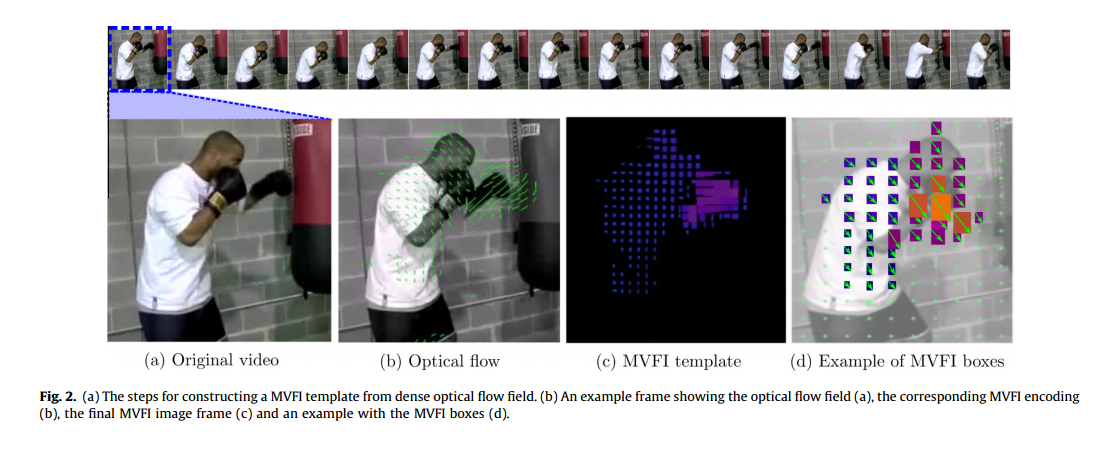
\includegraphics[width=1.0\linewidth]{Kap2/img/Selection_021.png}
\caption{cambiar}
\end{figure}

%\section{Comparación de los trabajos}

%\section{Consideraciones finales}

 

 



\chapter{Marco teórico}
Desarrollar métodos automáticos para analizar las acciones en videos es de particular importancia, primero se debe entender que acciones se dan en un video. El reconocimiento de acciones (patrones), que es el problema de asignar un video a un conjunto de clases de acción predefinidas, y la localización de acción, definida como la identificación de la localización spatio-temporal donde tiene lugar una acción, son dos de los temas fundamentales y muy estudiados en este contexto.

La mayoría de los marcos existentes para el reconocimiento de acciones consta de tres pasos principales: extracción de características, aprendizaje (entramiento de clases) para formar una representación de un video basado en las características extraídas y finalmente clasificación del video usando dicha representación.

En el primer paso, un conjunto de características, como STIP \cite{laptev2005space} o densa trayectorias \cite{wang2011action,
wang2013dense}, se extraen de un determinado video. Se supone que estas características codifican la información que es útil para el reconocimiento de la acción en una forma numérica (un vector). A continuación, las características extraídas se utilizan para formar una representación de un vídeo, que captura las acciones que se producen en el mismo. Tal representación puede ser tan simple como un histograma de los movimientos más frecuentes \cite{wang2011action,
wang2013dense} o un modelo semánticamente significativo. En el último paso, se aprende un modelo general para cada acción de interés usando la representación computarizada de un conjunto de vídeos de entrenamiento etiquetados.


\section{flujo óptico}
El flujo óptico es el patrón del movimiento aparente de los objetos de la imagen entre dos marcos consecutivos causados por el movimiento del objeto o de la cámara. Es un campo vectorial 2D donde cada vector es un vector de desplazamiento que muestra el movimiento de puntos desde el primer fotograma hasta el segundo. Considere la imagen de abajo (Imagen Cortesía: Artículo de Wikipedia sobre Flujo Óptico).

\subsection{Lucas-Kanadeen y flujo óptico}
OpenCV proporciona todo esto en una sola función, \textbf{cv2.calcOpticalFlowPyrLK ()}. El objetivos de esta técnica es crear una sencilla aplicacion para realizar un seguimiento a los puntos, usamos \textbf{cv2.goodFeaturesToTrack ()}. Tomamos el primer fotograma, detectamos algunos puntos de esquina de Shi-Tomasi (\ref{fig:datasetKth}) en él, entonces seguimos iterativamente esos puntos usando el flujo óptico de Lucas-Kanade. Para la función \textbf{cv2.calcOpticalFlowPyrLK ()} pasamos el fotograma anterior, los puntos anteriores y el fotograma siguiente. Devuelve los puntos siguientes junto con algunos números de estado que tiene un valor de 1 si se encuentra el siguiente punto, de lo contrario cero. Pasamos iterativamente los siguientes puntos como puntos anteriores en el siguiente paso. 
(figura \ref{fig:optical-flow1})

\begin{figure}[h!]

 % \centering
  \begin{subfigure}[]{0.4\linewidth}
      \centering 	  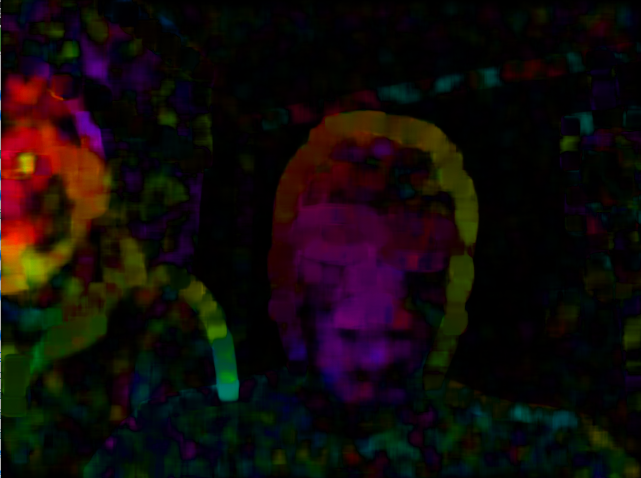
\includegraphics[width=0.4\textwidth]{Kap3/img/Dense_optical_flow_by_HSV_color_image.png}
  \caption{dense-optical-flow-HSV}     
  \label{fig:dense-optical-flow-HSV}
    \end{subfigure}
    
 % \centering
 %\hfill	
  \begin{subfigure}[]{0.4\linewidth}
      \centering     
 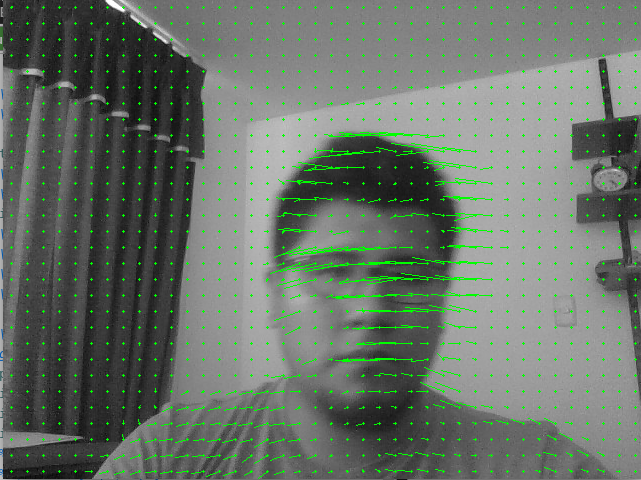
\includegraphics[width=0.4\textwidth]{Kap3/img/Dense_optical_flow_by_lines.png}
  \caption{Dense optical flow by lines}
      \label{fig:Dense_optical_flow_by_lines}
      \end{subfigure}

 % %%\centering
  \caption{Se muestra las 2 técnias de flujo optico.}
  \label{fig:optical-flow2}
\end{figure}




\begin{figure}[h!]

 % \centering
 %\hfill	
  \begin{subfigure}[]{0.4\linewidth}
      \centering
      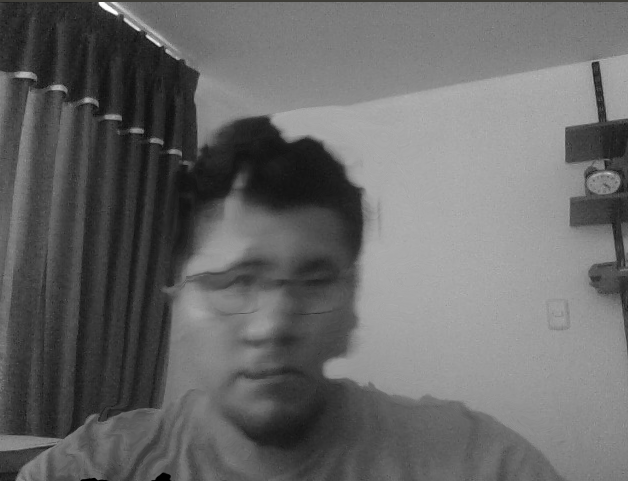
\includegraphics[width=0.4\textwidth]{Kap3/img/Dense_optical_flow_by_warped_image.png}
      \caption{Dense optical flow by warped image}
      \label{fig:Dense_optical_flow_by_warped_image}
  \end{subfigure}
  
   % \centering
  %\hfill	
    \begin{subfigure}[]{0.4\linewidth}
      \centering
      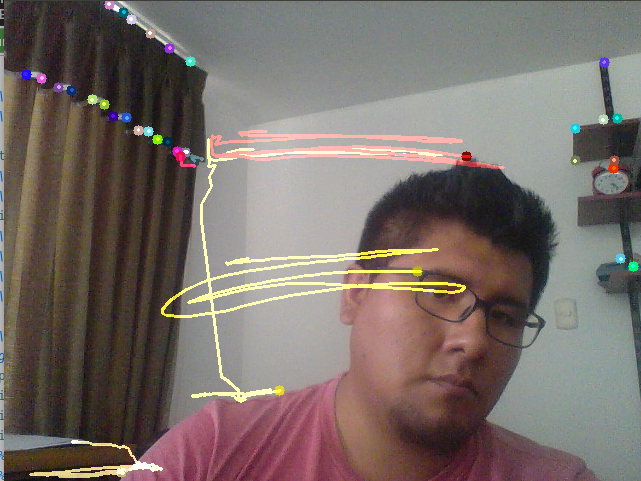
\includegraphics[width=0.4\textwidth]{Kap3/img/Lucas-Kanade_method.png}
      \caption{Lucas-Kanade method}
      \label{fig:Lucas-Kanade_method}
  \end{subfigure}
  
 % %%\centering
  \caption{Se muestra las 2 técnia de lucas kanade para flujo optico.}
  \label{fig:optical-flow1}
\end{figure}



\subsection{Dense Optical Flow}
Lucas-Kanade calcula el flujo óptico para un conjunto de características escasas(Figura \ref{fig:ShiTomasiCorner}). OpenCV proporciona otro algoritmo para encontrar el flujo óptico denso. Calcula el flujo óptico para todos los puntos en el \textit{frame}. Obtenemos una matriz de 2 canales con vectores de flujo óptico,\textbf{ $(u, v)$}. Encontramos su magnitud y dirección. Coloreamos el código para obtener una mejor visualización. La dirección corresponde al valor de tono de la imagen. La magnitud corresponde al plano Valor.(figura \ref{fig:optical-flow1})



\begin{figure}[h!]
\centering
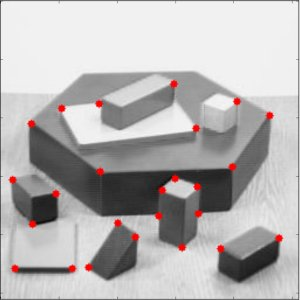
\includegraphics[width=0.6\linewidth]{Kap3/img/shitomasi_block_corner.jpg}
\caption{ en nuestro ejemplo, las esquinas detectadas usando el algoritmo Shi-Tomasi}
\label{fig:ShiTomasiCorner}
\end{figure}


\section{Dataset}

El actual \textit{dataset} \cite{data_set_KTH_baumann2016recognizing} contiene 6 tipos de acciones humanas (\textit{walking, jogging, running, boxing, hand waving y hand clapping}) cada una realizada muchas veces, exactamente por 25 sujetos en 4 diferentes scenarios: (FIGURA \ref{fig:datasetKth} )
\begin{itemize}
\item S1: al aire libre
\item S2: al aire libre con variacion de escala
\item S3: al aire libre con diferente ropa
\item S3: en un ambiente 
\end{itemize}

\begin{figure}[h!]
\centering
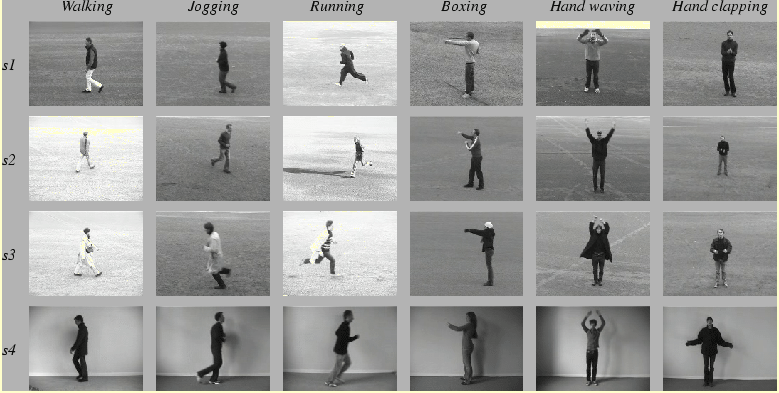
\includegraphics[width=0.6\linewidth]{Kap3/img/datasetKth.png}
\caption{ Se muestra algunos ejemplos de secuencias de un conjunto de datos con seis acciones realizadas por ocho personas diferentes. El conjunto de datos contiene $6*8*4=192$ secuencias y es un subconjunto de una base de datos más grande. Todas las secuencias se obtuvieron con una cámara estacionaria con la velocidad de fotogramas de 25fps y con el submuestreo de la resolución espacial a $160*120$ píxeles.}
\label{fig:datasetKth}
\end{figure}
    
Actualmente el \textit{dataset} contiene un total de 2391 secuencias de imagenes a lo largo de los diferentes videos. Las diferentes secuencias de imagenes fueron tomadas sobre ambientes homogeneos con una camara estatica \textit{"25fps frame rate"}, las secuencias usadas fueron reducidas a una resolucion de 160x120 pixeles y una duracion de 4 por segundo, en promedio.Para nuestros esperimentos reportados sobre \textit{"ICPR'04"} todas la secuencias de video fueron divididas con respecto a:
\begin{itemize}
\item training set (8 personas)
\item validation set (8 personas)
\item test set (9 personas)
\end{itemize}
	
Todas las secuencias de video usan el formato \textit{"AVI"} and estan disponibles (DIVX-compressed version). Hay 25x6x4=600 videos para cada combinación, 25 personas, 6 acciones y 4 escenarios. Cada archivo tiene informacion de las subsecuencias usadas en una secuencia. La subdivision para archivo esta señalado como \textit{"start-frame"} y \textit{"end-frame"} 



\subsection{Convolutional Neural Networks}
El primer trabajo que popularizó Redes Convolucionales en Visión por Computadora fue AlexNet, desarrollado por Alex Krizhevsky, Ilya Sutskever y Geoff Hinton. El AlexNet fue presentado al desafío de ImageNet ILSVRC en 2012 y superó significativamente al segundo subcampeón (error de los 5 primeros del 16\% en comparación con el subcampeón con 26\% de error). La Red tenía una arquitectura muy similar a LeNet, pero era más profunda, más grande y presentaba capas convolucionales apiladas unas encima de otras (anteriormente era común tener sólo una capa de CONV siempre seguida inmediatamente por una capa de POOL). \cite{link10-CS231n_Convolutional_Neural_Networks_for_Visual_Recognition}

%%%\chapter{Capítulo 3}
Se deben incluir tantos capítulos como se requieran; sin embargo, se recomienda que la tesis  o trabajo de investigación tenga un mínimo 3 capítulos y máximo de 6 capítulos (incluyendo las conclusiones).\\
%%%\chapter{Capítulo ...}
Se deben incluir tantos capítulos como se requieran; sin embargo, se recomienda que la tesis  o trabajo de investigación tenga un mínimo 3 capítulos y máximo de 6 capítulos (incluyendo las conclusiones).\\
%%%\chapter{Conclusiones y recomendaciones}
\section{Conclusiones}
Las conclusiones constituyen un capítulo independiente y presentan, en forma lógica, los resultados de la tesis  o trabajo de investigación. Las conclusiones deben ser la respuesta a los objetivos o propósitos planteados. Se deben titular con la palabra conclusiones en el mismo formato de los títulos de los capítulos anteriores (Títulos primer nivel), precedida por el numeral correspondiente (según la presente plantilla).\\

\section{Recomendaciones}
Se presentan como una serie de aspectos que se podrían realizar en un futuro para emprender investigaciones similares o fortalecer la investigación realizada. Deben contemplar las perspectivas de la investigación, las cuales son sugerencias, proyecciones o alternativas que se presentan para modificar, cambiar o incidir sobre una situación específica o una problemática encontrada. Pueden presentarse como un texto con características argumentativas, resultado de una reflexión acerca de la tesis o trabajo de investigación.\\
%%%\begin{appendix}
\chapter{Anexo: Nombrar el anexo A de acuerdo con su contenido}\label{AnexoA}
Los Anexos son documentos o elementos que complementan el cuerpo de la tesis o trabajo de investigaci\'{o}n y que se relacionan, directa o indirectamente, con la investigaci\'{o}n, tales como acetatos, cd, normas, etc.\\

\chapter{Anexo: Nombrar el anexo B de acuerdo con su contenido}
A final del documento es opcional incluir \'{\i}ndices o glosarios. \'{E}stos son listas detalladas y especializadas de los t\'{e}rminos, nombres, autores, temas, etc., que aparecen en el mismo. Sirven para facilitar su localizaci\'{o}n en el texto. Los \'{\i}ndices pueden ser alfab\'{e}ticos, cronol\'{o}gicos, num\'{e}ricos, anal\'{\i}ticos, entre otros. Luego de cada palabra, t\'{e}rmino, etc., se pone coma y el n\'{u}mero de la p\'{a}gina donde aparece esta informaci\'{o}n.\\

\chapter{Anexo: Nombrar el anexo C de acuerdo con su contenido}
MANEJO DE LA BIBLIOGRAF\'{I}A: la bibliograf\'{\i}a es la relaci\'{o}n de las fuentes documentales consultadas por el investigador para sustentar sus trabajos. Su inclusi\'{o}n es obligatoria en todo trabajo de investigaci\'{o}n. Cada referencia bibliogr\'{a}fica se inicia contra el margen izquierdo.\\

La NTC 5613 establece los requisitos para la presentaci\'{o}n de referencias bibliogr\'{a}ficas citas y notas de pie de p\'{a}gina. Sin embargo, se tiene la libertad de usar cualquier norma bibliogr\'{a}fica de acuerdo con lo acostumbrado por cada disciplina del conocimiento. En esta medida es necesario que la norma seleccionada se aplique con rigurosidad.\\

Es necesario tener en cuenta que la norma ISO 690:1987 (en Espa\~{n}a, UNE 50-104-94) es el marco internacional que da las pautas m\'{\i}nimas para las citas bibliogr\'{a}ficas de documentos impresos y publicados. A continuaci\'{o}n se lista algunas instituciones que brindan par\'{a}metros para el manejo de las referencias bibliogr\'{a}ficas:\\

\begin{center}
\centering%
\begin{tabular}{|p {7.5 cm}|p {7.5 cm}|}\hline
\arr{Instituci\'{o}n}&Disciplina de aplicaci\'{o}n\\\hline%
Modern Language Association (MLA)&Literatura, artes y humanidades\\\hline%
American Psychological Association (APA)&Ambito de la salud (psicolog\'{\i}a, medicina) y en general en todas las ciencias sociales\\\hline
Universidad de Chicago/Turabian &Periodismo, historia y humanidades.\\\hline
AMA (Asociaci\'{o}n M\'{e}dica de los Estados Unidos)&Ambito de la salud (psicolog\'{\i}a, medicina)\\\hline
Vancouver &Todas las disciplinas\\\hline
Council of Science Editors (CSE)&En la actualidad abarca diversas ciencias\\\hline
National Library of Medicine (NLM) (Biblioteca Nacional de Medicina)&En el \'{a}mbito m\'{e}dico y, por extensi\'{o}n, en ciencias.\\\hline
Harvard System of Referencing Guide &Todas las disciplinas\\\hline
JabRef y KBibTeX &Todas las disciplinas\\\hline
\end{tabular}
\end{center}

Para incluir las referencias dentro del texto y realizar lista de la bibliograf\'{\i}a en la respectiva secci\'{o}n, puede utilizar las herramientas que Latex suministra o, revisar el instructivo desarrollado por el Sistema de Bibliotecas de la Universidad Nacional de Colombia\footnote{Ver: www.sinab.unal.edu.co}, disponible en la secci\'{o}n "Servicios", opci\'{o}n "Tr\'{a}mites" y enlace "Entrega de tesis".

\end{appendix}%%%anexos
\addcontentsline{toc}{chapter}
{\numberline{}Bibliografía}
% Puede cambiarse por alguna otra como IEEE
\nocite{*}
\bibliographystyle{Encabezado/Biblio/plaindin_esp}
\bibliography{BibliMSc}
\end{document}